\documentclass[12pt, twoside]{article}
\usepackage[utf8]{inputenc}
\usepackage[english,russian]{babel}
\newcommand{\hdir}{.}
\usepackage{graphicx}
\usepackage{caption}
\usepackage{amssymb}
\usepackage{amsmath}
\usepackage{mathrsfs}
\usepackage{euscript}
\usepackage{upgreek}
\usepackage{array}
\usepackage{theorem}
\usepackage{graphicx}
\usepackage{subfig}
\usepackage{caption}
\usepackage{color}
\usepackage{url}
\usepackage{cite}
\usepackage{geometry}
\usepackage{tikz,fullpage}
\usepackage{enumerate}
\usepackage{amsmath}
\usepackage{hyperref}
\usepackage{cleveref}
\usepackage{autonum}
\usepackage{amsthm}


\newcommand{\bmatr}{{\mathbf{B}}}
\newcommand{\cmatr}{{\mathbf{C}}}
\newcommand{\hmatr}{{\mathbf{H}}}
\newcommand{\fmatr}{{\mathbf{F}}}
\newcommand{\mmatr}{{\mathbf{M}}}
\newcommand{\xmatr}{{\mathbf{X}}}
\newcommand{\pmatr}{{\mathbf{P}}}
\newcommand{\xmatrt}{{\tilde{\mathbf{X}}}}
\newcommand{\imatr}{{\mathbf{I}}}
\newcommand{\vmatr}{{\mathbf{V}}}
\newcommand{\wmatr}{{\mathbf{W}}}
\newcommand{\umatr}{{\mathbf{U}}}
\newcommand{\zmatr}{{\mathbf{Z}}}
\newcommand{\zmatrt}{{\tilde{\mathbf{Z}}}}
\newcommand{\Tmatr}{\mathbf{T}}
\newcommand{\lambdamatr}{{\mathbf{\Lambda}}}
\newcommand{\phimatr}{\mathbf{\Phi}}
\newcommand{\sigmamatr}{\mathbf{\Sigma}}
\newcommand{\thetamatr}{\boldsymbol{\Theta}}

\newcommand{\ab}{{\mathbf{a}}}
\newcommand{\bb}{{\mathbf{b}}}
\newcommand{\cb}{{\mathbf{c}}}
\newcommand{\db}{{\mathbf{d}}}
\newcommand{\eb}{{\mathbf{e}}}
\newcommand{\fb}{{\mathbf{f}}}
\newcommand{\gb}{{\mathbf{g}}}
\newcommand{\hb}{{\mathbf{h}}}
\newcommand{\mb}{{\mathbf{m}}}
\newcommand{\pb}{{\mathbf{p}}}
\newcommand{\qb}{{\mathbf{q}}}
\newcommand{\rb}{{\mathbf{r}}}
\newcommand{\tb}{{\mathbf{t}}}
\newcommand{\ub}{{\mathbf{u}}}
\newcommand{\vb}{{\mathbf{v}}}
\newcommand{\wb}{{\mathbf{W}}}
\newcommand{\xb}{{\mathbf{x}}}
\newcommand{\xt}{{\tilde{x}}}
\newcommand{\xbt}{\tilde{{\mathbf{x}}}}
\newcommand{\yb}{{\mathbf{y}}}
\newcommand{\zb}{{\mathbf{z}}}
\newcommand{\zt}{{\tilde{z}}}
\newcommand{\zbt}{{\tilde{\mathbf{z}}}}
\newcommand{\mub}{{\boldsymbol{\mu}}}
\newcommand{\alphab}{{\boldsymbol{\alpha}}}
\newcommand{\thetab}{{\boldsymbol{\theta}}}
\newcommand{\iotab}{\boldsymbol{\iota}}
\newcommand{\zetab}{\boldsymbol{\zeta}}
\newcommand{\xib}{\boldsymbol{\xi}}
\newcommand{\xibt}{\tilde{\boldsymbol{\xi}}}
\newcommand{\xit}{\tilde{\xi}}
\newcommand{\betab}{{\boldsymbol{\beta}}}
\newcommand{\phib}{{\boldsymbol{\phi}}}
\newcommand{\psib}{{\boldsymbol{\psi}}}
\newcommand{\gammab}{{\boldsymbol{\gamma}}}
\newcommand{\lambdab}{{\boldsymbol{\lambda}}}
\newcommand{\varepsilonb}{{\boldsymbol{\varepsilon}}}
\newcommand{\pib}{{\boldsymbol{\pi}}}
\newcommand{\sigmab}{{\boldsymbol{\sigma}}}


\newcommand{\scl}{s_{\mathsf{c}}}
\newcommand{\shi}{s_{\mathsf{h}}}
\newcommand{\shib}{\mathbf{s}_{\mathsf{h}}}
\newcommand{\MOD}{M}
\newcommand{\entr}{\mathsf{H}}
\newcommand{\REG}{\Omega}
\newcommand{\Mquol}{V}
\newcommand{\prob}{p}
\newcommand{\expec}{\mathsf{E}}

\newcommand{\xo}{{\overline{x}}}
\newcommand{\Xo}{{\overline{x}}}
\newcommand{\yo}{{\overline{y}}}

\newcommand{\xbo}{{\overline{\mathbf{x}}}}
\newcommand{\Xbo}{{\overline{\mathbf{X}}}}

\newcommand{\Amc}{{\mathcal{A}}}
\newcommand{\Bmc}{{\mathcal{B}}}
\newcommand{\Cmc}{{\mathcal{C}}}
\newcommand{\Jmc}{{\mathcal{J}}}
\newcommand{\Imc}{{\mathcal{I}}}
\newcommand{\Kmc}{{\mathcal{K}}}
\newcommand{\Lmc}{{\mathcal{L}}}
\newcommand{\Mmc}{{\mathcal{M}}}
\newcommand{\Nmc}{{\mathcal{N}}}
\newcommand{\Pmc}{{\mathcal{P}}}
\newcommand{\Tmc}{{\mathcal{T}}}
\newcommand{\Vmc}{{\mathcal{V}}}
\newcommand{\Wmc}{{\mathcal{W}}}


\newcommand{\T}{^{\text{\tiny\sffamily\upshape\mdseries T}}}
\newcommand{\deist}{\mathbb{R}}
\newcommand{\ebb}{\mathbb{E}}

\newcommand{\Amatr}{\mathbf{A}}
\newcommand{\X}{\mathbf{X}}
\newcommand{\Z}{\mathbf{Z}}
\newcommand{\Umatr}{\mathbf{U}}
\newcommand{\zetavec}{\boldsymbol{\zeta}}

\newcommand{\M}{\mathbf{M}}
\newcommand{\x}{{\mathbf{x}}}
\newcommand{\z}{{\mathbf{z}}}
\newcommand{\ical}{{\mathcal{I}}}
\newcommand{\tvec}{{\mathbf{t}}}
\newcommand{\xvec}{{\mathbf{x}}}
\newcommand{\zvec}{{\mathbf{z}}}
\newcommand{\bvec}{{\mathbf{b}}}
\newcommand{\qvec}{{\mathbf{z}}}
\newcommand{\pvec}{{\mathbf{p}}}
\newcommand{\wvec}{{\mathbf{W}}}
\newcommand{\rvec}{{\mathbf{r}}}
\newcommand{\thetavec}{{\mathbf{\theta}}}
\newcommand{\y}{{\mathbf{y}}}
\newcommand{\g}{{\mathbf{g}}}
\newcommand{\w}{{\mathbf{W}}}
\newcommand{\wm}{{\mathbf{w}}}
\newcommand{\m}{{\mathbf{m}}}

\renewcommand{\baselinestretch}{1.3} 

\theoremstyle{definition}
\DeclareMathOperator*{\argmin}{arg\,min}
%\graphicspath{ {fig/} }

\newtheorem*{theorem*}{Теорема}
\newtheorem{theorem}{Теорема}

\newtheorem*{definition*}{Определение}
\newtheorem{definition}{Определение}


\begin{document}
\selectlanguage{russian}


\section{Теорема Цыбенко об аппроксимации}
\begin{definition*}
$\sigma: \mathbb{R} \to \mathbb{R}$ называется сигмоидной функцией, если пределы $\lim_{x \to \infty} \sigma(x)$, $\lim_{x \to -\infty} \sigma(x)$ существуют и $\lim_{x \to \infty} \sigma(x) = 1, \lim_{x \to -\infty} \sigma(x) = 0$. $\sigma$ должна быть непрерывной.
\end{definition*}
Например 
$$\sigma(x) = \frac{1}{1+\exp{-x}}$$
является сигмоидной функцией, также сигмоидой является 
\[ \begin{cases} 
      1, x\geqslant0 \\
      0, x<0 \\
   \end{cases}
\]

Теорема доказана Джорджем Цыбенко в 1989 году и утверждает, что нейронная сеть с одним скрытым слоем может аппроксимировать любую непрерывную функцию многих переменных с любой точностью. Условиями являются: достаточное количество нейронов скрытого слоя и удачный подбор параметров. В \cite{bib_1} показано, что сети с активационной функцией ReLU с шириной n + 1 достаточны для аппроксимации любой непрерывной функции n-мерных входных переменных.
\begin{theorem*}
Если $\sigma(x)$ это ограниченнная сигмоидная функция, и $f(x)$ это непрерывная функция на $(-\infty,\infty)$ для которой $\lim_{x \to -\infty} \f(x) = A$ и $\lim_{x \to \infty} \f(x) = B$, где $A,B$ - константы, то для любого $\varepsilon>0$ существуют $N, c_{i}, y_{i}, \theta_{i}$ такие что
$$|f(x)-\sum\limits_{i=1}^Nc_i\sigma(y_{i}x+\theta_{i})|<\varepsilon$$
для всех $x\in(-\infty,\infty)$.
\end{theorem*}

\begin{proof}

Доказательство является конструктивным. Из предположения, для любого $\varepsilon>0$ мы можем найти $M>0$ такое что $|f(x)-A|<\frac{\varepsilon}{4}$ если  $x<-M$; $|f(x)-B|<\frac{\varepsilon}{4}$ если $x>M$; и  $|f(x')-f(x")|<\frac{\varepsilon}{4}$ если  $|x'|\leq M$, $|x''|\leq M$ и $|x'-x''|\leq \frac{1}{M}$.

Разделим $[-M;M]$ на $2M^2$ равных отрезков, каждый длины $\frac{1}{M}$, и положим $$-M=x_0<x_1<\dots<x_{M^2}=0<x_{M^2+1}<\dots<x_{2M^2}=M$$
Пусть $t_i=\frac{1}{2}(x_i+x_{i+1})$ будет центром интервала $[x_i,x_{i+1}]$. Теперь построим функцию \begin{equation}\label{eq2}
g(x) = f(-M) + \sum\limits_{i=1}^N[f(x_{i}) - f(x_{i-1})]\sigma(K(x-t_{i-1}))
\end{equation}
где $N=2M^2$.

Исходя из предположения, существует $W>0$ такое что если  $u>W$ тогда $|\sigma(u)-1|<\frac{1}{M^2}$, если $u<-W$ тогда $|\sigma(u)|<\frac{1}{M^2}$. Положим $K>0$ так чтобы $K\frac{1}{2M}>W$.

Мы утверждаем, что $|f(x)-g(x)|<\varepsilon$ выполняется для всех $x\in(-\infty,\infty)$.
\paragraph{(i)} Если $x<-M$, тогда $|f(x)-f(-M)|<\frac{\varepsilon}{2}$,
\begin{equation}\label{eq3}
|g(x)-f(-M)|\leq\sum\limits_{i=1}^{2M^2}|f(x_{i}) - f(x_{i-1})||\sigma(K(x-t_{i-1}))|<\sum\limits_{i=1}^{2M^2}\frac{\varepsilon}{4}\frac{1}{M^2}=\frac{\varepsilon}{2}
\end{equation}
следовательно $|f(x)-g(x)|<\varepsilon$.
\paragraph{(ii)} Если $x>M$, тогда $|f(x)-f(M)|<\frac{\varepsilon}{2}$,
\begin{equation}\label{eq4}
|g(x)-f(M)|\leq\sum\limits_{i=1}^{2M^2}|f(x_{i}) - f(x_{i-1})||\sigma(K(x-t_{i-1}))-1|<\sum\limits_{i=1}^{2M^2}\frac{\varepsilon}{4}\frac{1}{M^2}=\frac{\varepsilon}{2}
\end{equation}
следовательно $|f(x)-g(x)|<\varepsilon$.
\paragraph{(iii)} Рассмотрим $x\in[x_{k-1},x_k]$, тогда $|x-t_{i-1}|\leq\frac{1}{2M}$ если $i=k$; $|x-t_{i-1}|>\frac{1}{2M}$ если $i\neq k$. Кроме того, если $i<k$ тогда $K(x-t_{i-1})>W$, и следовательно $|\sigma(K(x-t_{i-1}))-1|<\frac{1}{M^2}$; если $i>k$, тогда $K(x-t_{i-1})<-W$, и следовательно $|\sigma(K(x-t_{i-1}))|<\frac{1}{M^2}$.

В результате мы имеем
\begin{equation}\label{eq5}
|g(x)-f(-M) - [f(x_k)-f(x_{k-1})]\sigma(K(x-t_{k-1})) -\sum\limits_{i=1}^{k-1}[f(x_{i}) - f(x_{i-1})]|\leavevmode\\\leq\sum\limits_{i=1}^{k-1}|f(x_{i}) - f(x_{i-1})||\sigma(K(x-t_{k-1}))-1|+\sum\limits_{i=k+1}^{2M^2}|f(x_{i})-f(x_{i-1})||\sigma(K(x-t_{i-1}))|\leavevmode\\\leq\sum\limits_{i=1}^{k-1}\frac{\varepsilon}{4}\frac{1}{M^2}+\sum\limits_{i=k+1}^{2M^2}\frac{\varepsilon}{4}\frac{1}{M^2}<\frac{\varepsilon}{2}
\end{equation}

Ясно, что
\begin{equation}\label{eq6}
f(-M) + [f(x_k)-f(x_{k-1})]\sigma(K(x-t_{k-1})) +\sum\limits_{i=1}^{k-1}[f(x_{i}) - f(x_{i-1})]|
= f(x_{k-1}) + [f(x_k)-f(x_{k-1})]\sigma(K(x-t_{k-1}))
\end{equation}

и объединив это с предыдущим неравенством, получаем 
\begin{equation}\label{eq7}
|g(x)-f(x)|<\frac{\varepsilon}{2}+|f(x)-f(x_{k-1})|+|f(x_k)-f(x_{k-1})||\sigma(K(x-t_{k-1}))|<\frac{\varepsilon}{2}+\frac{\varepsilon}{4}+\frac{\varepsilon}{4}<\varepsilon.
\end{equation}
Здесь мы предположили, без потери общности, что $\sigma(x)\leq1$ для всех $x\in(-\infty,\infty)$.

\begin{comment}
Для того, чтобы закончить доказательство теоремы, нам необходимо только позаботиться о $f(-M)$, или дополнительно показать что консанта 1 может быть аппроксимирована с помощью линейной комбинации $\sum c_i\sigma(y_{i}x+\theta_{i})$.
Пусть $N,M,x_{i},t_{i},K$ будут теми же константами, что и ранее, тогда это легко подтвердить что 
\begin{equation}\label{eq8}
\frac{1}{N}\sum\limits_{i=1}^{N}[\sigma(K(x-t_{i-1}))+\sigma(-K(x-t_{i-1}))]
\end{equation}
\end{comment}
\end{proof}
Таким образом, любую непрерывную функцию нескольких
переменных можно с любой точностью реализовать с помощью обычного трехслойного перцептрона с достаточным количеством нейронов в скрытом слое.

\section{Теорема Колмогорова}
\begin{theorem*}
Каждая непрерывная функция n переменных, заданная на единичном кубе n-мерного пространства $E_n$, представима в виде
\begin{equation}\label{eq9}
f(x_1,x_2,\dots,x_n) = \sum\limits_{q=1}^{2n+1}h_q[\sum\limits_{p=1}^{n}\varphi_p^{q}(x_p)],
\end{equation}
\end{theorem*}
где функции $h_q(u)$ — непрерывны, а функции $\varphi_p^{q}(x_p)$, кроме того, еще
стандартны, т.е. не зависят от выбора функции $f$; в частности, каждая непрерывная функция двух переменных представима в виде
\begin{equation}\label{eq10}
f(x,y) = \sum\limits_{q=1}^{5}h_q[\varphi_q(x)+\psi_{q}(y)].
\end{equation}
При $n=3$ из \eqref{eq9} следует 
\begin{equation}\label{eq11}
f(x,y,z) = \sum\limits_{q=1}^{7}h_q[\varphi_q(x)+\psi_{q}(y)+\chi_{q}(z)] = \sum\limits_{q=1}^{7}F_{q}[g_q(x,y),z]
\end{equation}
где положено 
\begin{equation}\label{eq12}
F_{q}(u,z) = h_{q}[u+\chi_{q}(z)], g_{q} = \varphi_{q}(x)+\psi_{q}(y).
\end{equation}
Так как все идеи доказательства отчетливо проявляются уже в случае $n=2$, то мы будем говорить лишь о представлении \eqref{eq10} произвольной непрерывной функции $f(x,y)$ двух переменных \textit{х} и \textit{у}. Возможность такого представления доказывается в несколько этапов.
\paragraph{(i)} «Внутренние» функции $\varphi_q(x)$ и $\psi_{q}(y)$ представления \eqref{eq10} совершенно не зависят от разлагаемой функции $f(x,y)$.
\begin{figure}[ht!]
  \centering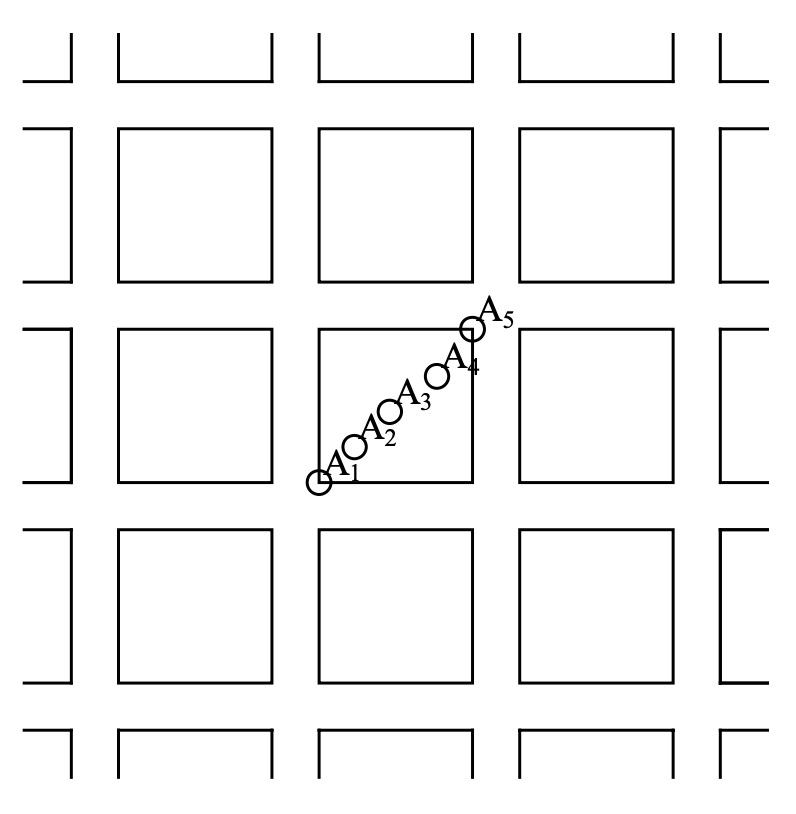
\includegraphics[scale=0.6]{kvartal.png}
  \label{fig:boat5}
\end{figure}
Для определения этих функций нам понадобятся некоторые предварительные построения. Рассмотрим изображенный на рис. 1 «город» — систему одинаковых <<кварталов>> (непересекающихся замкнутых квадратов) разделенных узкими <<улицами>> одной и той же ширины. Уменьшим гомотетично наш <<город>> в $N$ раз; за центр гомотетии можно принять, например, точку $A_1$ - мы получим новый <<город>>, который будем называть <<городом ранга 2>>. <<Город ранга 3>> точно также получается из <<города ранга 2>> гомотетичным уменьшением с коэффициентом гомотетии $\frac{1}{N}$; <<город ранга 4>> получается гомотетичным уменьшением в $N$ раз раз <<города ранга 3>> и т.д. Вообще <<город ранга $k$>> получается из исходного <<города>> (который мы будем называть <<городом первого ранга>>) гомотетичным уменьшением в $N^k$ раз (с центром гомотетии в $A_1$; впрочем, выбор центра гомотетии не существенен для дальнейшего).

Построенную систему <<городов>> мы назовем 1-й системой. <<Город первого ранга $q$-й системы>> ( $q=2,\dots,5$) получается из изображенного на рис. 1 <<города>> при помощи параллельного переноса, совмещающего точку $A_1$ с точкой $A_q$. Нетрудно понять, что <<улицы>> <<города>> можно выбрать настолько узкими, что каждая точка плоскости будет покрыта по крайней мере тремя кварталами наших пяти <<городов первого ранга>>. Точно так же <<город $k$-го ранга>> $q$-й системы ($k=2,3,\dots;q=2,\dots,5$) получается из <<города $k$-го ранга 1-й системы>> параллельным переносом, переводящим точку $A_1^k$ в точку $A_q^k$, где $A_1^k$ и $A_q^k$ получаются из точек $A_1$ и $A_q$ гомотетией, переводящей <<город первого ранга>> 1-й системы (т.е. наш исходный <<город>>) в <<город $k$-го ранга>> той же системы; при этом каждая точка плоскости будет принадлежать кварталам по крайней мере трех из пяти "городов" любого фиксированного ранга  $k$.

Функцию 
\begin{equation}\label{eq13}
\Phi_{q}(x,y) = \varphi_{q}(x)+\psi_{q}(y) (q=1,2,\dots,5)
\end{equation}
мы определим теперь так, чтобы она разделяла любые два <<квартала>> каждого <<города>> системы $q$, т.е. чтобы множество значений, принимаемых $\Phi_{q}(x,y)$ на определенном <<квартале>> <<города $k$-го ранга>> (здесь $k$ - произвольное фиксированное число) $q$-й системы, не пересекалось с множеством значений, принимаемых $\Phi_{q}(x,y)$ на любом другом <<квартале>> того же <<города>>. При этом нам, разумеется, будет достаточно рассматривать функцию $\Phi_{q}(x,y)$ на единичном квадрате (а не на всей плоскости).

Для того, чтобы функция $\Phi_{q}(x,y) = \varphi_{q}(x)+\psi_{q}(y)$ разделяла <<кварталы>> <<города первого ранга>>, можно потребовать, например, чтобы $\varphi_{q}(x)$ на проекциях <<кварталов>> <<города>> на ось \textit{x} весьма мало отличалась от различных целых чисел, а $\psi_{q}(y)$ на проекциях <<кварталов>> на ось \textit{y} весьма мало отличалась от различных кратных $\sqrt2$ (ибо $m+n\sqrt2 =m^{'}+n^{'}\sqrt2$ при целых $m, n, m', n'$, лишь если $m=m',n=n'$). При этом наложенные условия не определяют пока еще, разумеется, функций $\varphi_{q}(x)$ и $\psi_{q}(y)$ (на <<улицах>> функция $\Phi_{q}(x,y) = \varphi_{q}(x)+\psi_{q}(y)$ вообще пока может задаваться совершенно произвольно); используя это, можно подобрать границы значений $\varphi_{q}(x)$ и $\psi_{q}(y)$ на <<кварталах>> <<города второго ранга>> так, чтобы функция $\Phi_{q}(x,y) = \varphi_{q}(x)+\psi_{q}(y)$ разделяла не только <<кварталы>> <<города 1 -го ранга>>, но и <<кварталы>> <<города 2 -го ранга>>. Намеченную программу можно осуществить, если N достаточно велико (так что кварталы последующих рангов не соединяют кварталы предыдущих). А.Н. Колмогоров выбрал $N=18$. Привлекая подобным же образом к рассмотрению "города" последующих рангов и уточняя каждый раз значения функций $\varphi_{q}(x)$ и $\psi_{q}(y)$, мы в пределе получим непрерывные функции $\varphi_{q}(x)$ и $\psi_{q}(y)$ (можно даже потребовать, чтобы они были монотонными), удовлетворяющие поставленным условиям

\paragraph{(ii)} Функции $h_q(u)$ разложения \eqref{eq10}, напротив того, существенно зависят от исходной функции $f(x,y)$. Для построения этих функций докажем прежде всего, что \textit{любую непрерывную функцию  $f(x,y)$ двух переменных $x$ и $y$, заданную на единичном квадрате, можно представить в виде}
\begin{equation}\label{eq14}
f(x,y) = \sum\limits_{q=1}^{5}h_q^{(1)}(\Phi_q(x,y))+f_{1}(x,y),
\end{equation}
где $\Phi_q(x,y) = \varphi_q(x)+\psi_{q}y$ - функции, построенные выше и  
\begin{equation}\label{eq15}
M_1=\text{max}|f_{1}(x,y)|\leq\frac{5}{6}\text{max}|f(x,y)|=\frac{5}{6}M,
\end{equation}
\begin{equation}\label{eq16}
\text{max}|h_{q}^{(1)}(\Phi_q(x,y))|\leq\frac{1}{3}M, q = 1,\dots,5.
\end{equation}
Выберем ранг $k$ столь большим, чтобы колебание (т.е. разность наибольшего и наименьшего значений) функции $f(x,y)$ на каждом <<квартале>> любого из <<городов ранга $k$>> не превосходило ${\frac{1}{6}}M$; это, разумеется, возможно, так как с ростом ранга $k$ размеры <<кварталов>> уменьшаются неограниченно. Далее, пусть $p_1^{(ij)}$ - определенный <<квартал>> <<города 1 -й системы>> (и выбранного ранга $k$ ); в таком случае (непрерывная) функция $\Phi_1(x,y)$ принимает на этом <<квартале>> значения, принадлежащие определенному сегменту $\Delta_1^{(ij)}$ числовой оси (причем в силу определения функции $\Phi_1$ этот сегмент не пересекается с сегментами значений, принимаемых $\Phi_1$ на всех других <<кварталах>>). Положим теперь функцию $h_1^{(1)}$ на сегменте $\Delta_1^{(ij)}$ постоянной, равной $\frac{1}{3}$ значения, принимаемого функцией $f(x,y)$ в какой-либо (безразлично какой) внутренней точке $M_1^{(ij)}$ квартала $p_1^{(ij)}$ (эту точку можно назвать <<центром квартала>>). Таким же образом мы определим функцию $h_1^{(1)}$ на любом другом из сегментов, задаваемых значениями функции $\Phi_1(x,y)$ на <<кварталах>> <<города $k$-го ранга>> 1 -й системы; при этом все значения $h_1^{(1)}$ будут по модулю не превосходить ${\frac{1}{3}}M$ (ибо значение $f(x,y)$ в <<центре>> любого <<квартала>> по модулю не превосходит $M$). Доопределим теперь функцию $h_1^{(1)}(u)$ при тех значениях аргумента $u$, при каких она еще не определена, произвольно, с тем лишь, чтобы она была непрерывна и чтобы выполнялось неравенство \eqref{eq16}; совершенно аналогично определим и все остальные функции  $h_q^{(1)}(u) (q=2,\dots,5 )$.

Докажем теперь, что разность 
\begin{equation}\label{eq17}
f_1(x,y)=f(x,y)-\sum\limits_{q=1}^5 {h_q^{(1)}(\Phi_q(x,y))} 
\end{equation}
довлетворяет условию \eqref{eq15}, т.е. что
\begin{equation}\label{eq18}
\left|{f_1 (x_0 ,y_0 )} \right|\le \frac{5}{6}M,
\end{equation}
где $(x_0,y_0)$ - произвольная точка единичного квадрата.  Эта точка (как и все точки плоскости) принадлежит по крайней мере трем кварталам <<городов ранга $k$>>; поэтому заведомо найдутся такие три из пяти функций $h_1^{(1)}(\Phi_q (x,y))$, которые принимают в точке $(x_0 ,y_0 )$ значение, равное ${\frac{1}{3}}$ значения $f(x,y)$ в <<центре>> соответствующего <<квартала>>, т.е. отличающееся от ${\frac{1}{3}}{f(x_0 ,y_0 )}$ не более чем на ${\frac{1}{18}}{\rm{M}}$ (ибо колебание $f(x,y)$ на каждом квартале не превосходит ${\frac{1}{6}}{\rm{M}}$ ); сумма этих трех значений $h_q^{(1)} (\Phi_q (x_0 ,y_0 ))$ будет отличаться от $f(x_0 ,y_0 )$ по модулю не более чем на ${\frac{1}{6}}{\rm{M}}$. А так как каждое из оставшихся двух чисел $h_q^{(1)} (\Phi_q (x_0 ,y_0 ))$ в силу (3) по модулю не превосходит ${\frac{1}{3}}{\rm{M}}$ то мы получаем:
\begin{equation}\label{eq19}
\left|{f_1 (x_0 ,y_0 )} \right|=\left|{f(x_0 ,y_0 )-\sum\limits_{q=1}^5 {h_q^{(1)}(\Phi_q (x_0 ,y_0 ))}}\right|\leq\frac{1}{6}M+\frac{2}{3}M=\frac{5}{6}M ,
\end{equation}
что и доказывает \eqref{eq15}.
Применим теперь то же разложение (3) к входящей в (3) функции $f_1 (x,y)$; мы получим:
\begin{equation}\label{eq20}
f_1(x,y)=\sum\limits_{q=1}^5 {h_q^{(2)} (\Phi_q (x,y))+f_2 (x,y)} 
\end{equation}
или
\begin{equation}\label{eq21}
f(x,y)=\sum\limits_{q=1}^5 {h_q^{(1)} (\Phi_q (x,y))}+\sum\limits_{q=1}^5 {h_q^{(2)} (\Phi_q (x,y))}+f_2 (x,y),
\end{equation}
где
\begin{equation}\label{eq22}
M_2 =\max \left|{f_2 (x,y)} \right|\le \frac{5}{6}M_1 =\left( {\frac{5}{6}} \right)^2 M,
\end{equation}
и
\begin{equation}\label{eq22}
\max \left|{h_q^{(2)} (\Phi_q (x,y))} \right|\leq \frac{1}{3}M_1 \leq \frac{1}{3} \cdot \frac{5}{6}M
(q=1,2,\dots,5 ).
\end{equation}
Затем мы применим разложение \eqref{eq14} к полученной функции $f_2(x,y)$ и т.д.; после $n$ -кратного применения этого разложения мы будем иметь:
\begin{equation}\label{eq23}
f(x,y)=\sum\limits_{q=1}^5 {h_q^{(1)} (\Phi_q (x,y))}+\sum\limits_{q=1}^5 {h_q^{(2)} (\Phi_q (x,y))}+f_2 (x,y)+\dots
\dots+\sum\limits_{q=1}^5 {h_q^{(n - 1)} (\Phi_q (x,y))}+f_n (x,y)
\end{equation}
где
\begin{equation}\label{eq24}
M_n =\max \left|{f_n (x,y)} \right|\le \left( {\frac{5}{6}} \right)^n M
\end{equation}
и
\begin{equation}\label{eq25}
\max \left|{h_q^{(s)} (\Phi_q (x,y))} \right|\le \frac{1}{3} \cdot \left( {\frac{5}{6}} \right)^{s - 1} M ( q=1,2,...,5;s=1,2,...,n - 1 ).
\end{equation}
Последние оценки показывают, что при $n \to \infty$ получим:
\begin{equation}\label{eq26}
f(x,y)=\sum\limits_{q=1}^5 {h_q^{(1)} (\Phi_q (x,y))}+\sum\limits_{q=1}^5 {h_q^{(2)} (\Phi_q (x,y))}+f_2 (x,y)+...
...+\sum\limits_{q=1}^5 {h_q^{(n)} (\Phi_q (x,y))}+...
\end{equation}
где стоящий справа бесконечный ряд сходится равномерно; также и каждый из пяти рядов
\begin{equation}\label{eq26}
h_q^{(1)} (\Phi_q (x,y))+h_q^{(2)} (\Phi_q (x,y))+h_q^{(n)} (\Phi_q (x,y))+... ( q=1,2,...,5
 )
\end{equation}
сходится равномерно, что позволяет ввести обозначения
\begin{equation}\label{eq27}
h_q (u)=h_q^{(1)}+h_q^{(2)}+...+h_q^{(n)}+... ( q=1,2,...,5 ).
\end{equation}
Итак, окончательно получаем:
\begin{equation}\label{eq28}
f(x,y)=\sum\limits_{q=1}^5 {h_q (\Phi_q (x,y))} =\sum\limits_{q=1}^5 h_q \left[{\varphi_q (x)+\psi_q (y)} \right]
,
\end{equation} то есть требуемое разложение (2).

Таким образом, любую непрерывную
функцию n переменных можно получить с помощью операций сложения, умножения и суперпозиции из непрерывных функций одного переменного. Так существуют ли функции многих переменных? В каком-то смысле - да, в каком-то - нет. Все непрерывные функции многих переменных могут быть получены из непрерывных функций одного переменного с помощью линейных операций и суперпозиции.

Выражение \eqref{eq9} имеет структуру нейронной сети с одним скрытым слоем из 2n+1 нейронов. Теорема Колмогорова показала принципиальную возможность реализации сколь угодно сложных зависимостей с помощью относительно простой нейронной сети,
называемой многослойным персептроном. 

\section{Теорема о глубоких нейросетях}
Эта теорема об аппроксимирующей силе глубины нейронных сетей с активационной функцией ReLU и ограниченной шириной. Особенно интересеы следующие вопросы: какова минимальная ширина $\omega_\min(d)$, чтобы сети ReLU ширины $\omega_\min(d)$ (и произвольной глубины) могли сколь угодно хорошо приближать любую непрерывную функцию на единичном кубе $[0,1]^d$ ? Что можно сказать о глубине сети, необходимой для аппроксимации заданной функции, для сетей ReLU вблизи этой минимальной ширины?

Для начала введем несколько обозначений
\begin{equation}\label{eq100}
||f||_{C_0}:=\sup_{x\in [0,1]^d} |f(x)|
\end{equation}
Далее обозначим через
\begin{equation}\label{eq101}
\omega_f(\varepsilon):=\sup\{|f(x)-f(y)| , |x-y|\leq\varepsilon\}
\end{equation}
модуль непрерывности функции $f$. Определим нейронную сеть
сеть с активационной функцией ReLU, размерностью входа $d_in$, шириной скрытого слоя $\omega$, глубиной $n$ и размером выхода $d_out$.
\begin{equation}\label{eq102}
ReLU\circ A_n \circ\dots\circ ReLU \circ A_1
\end{equation}
где
\begin{equation}\label{eq103}
A_j:\mathbb{R}^\omega\rightarrow\mathbb{R}^\omega, j=2,\dots,n-1, 
A_1:\mathbb{R}^{d_in}\rightarrow\mathbb{R}^\omega, A_n:\mathbb{R}^{\omega}\rightarrow\mathbb{R}^{d_out}
\end{equation}
\begin{equation}\label{eq104}
ReLU(x_1,\dots,x_m) = (\max\{0,x_1\},\dots,\max\{0,x_m\})
\end{equation}
Обозначим такую сеть за $\mathbb{N}$ и запишем
\begin{equation}\label{eq105}
f_{\mathbb{N}}(x) = ReLU\circ A_n \circ\dots\circ ReLU \circ A_1\circ ReLU \circ A_1(x)
\end{equation}
\begin{theorem*} Пусть $n \geq 1$ и $f: [0,1]^n \rightarrow \mathbb{R}_+$~--- положительная функция с нормой $||f||_{C_0} = 1$. Тогда: 
\begin{enumerate}
    \item Если $f$~--- непрерывная, то существует последовательность нейронных сетей прямого распространения $\mathcal{N}_k$ c функциями активации ReLU, размер входного слоя~--- $n$, скрытого~--- $n+2$, выходного слоя~--- $1$ такие, что 
    \begin{equation}\label{eq94}
        \underset{k \rightarrow \infty}\lim||f - f_{\mathcal{N}_k}||_{C^0} = 0.
    \end{equation}
    В частности, $\omega_{\min}(n) \leq n + 2$ Кроме того, если зафиксировать $\varepsilon > 0$ и взять модуль непрерывности функции $f$ $\omega_f(\varepsilon)$, то найдется нейронная сеть прямого распространения $\mathcal{N}_{\varepsilon}$ с функциями активации ReLU , размерами входного слоя $n$, скрытого слоя~--- $n+3$, выходного слоя~--- $1$, и 
    \begin{equation}\label{eq95}
        \textnormal{depth}(\mathcal{N}_{\varepsilon}) = \frac{2 \cdot n!}{\omega_f(\varepsilon)^n}.
    \end{equation}
    такая, что \begin{equation}
        ||f - f_{\mathcal{N}_{\varepsilon}}||_{C_0} \leq \varepsilon.
    \end{equation} \\
    \item Если $f$~--- выпуклая, то существует последовательность нейронных сетей прямого распространения  $\mathcal{N}_{m}$ c функциями активации ReLU, размерами входного слоя~--- $n$, скрытого слоя~--- $n+1$, и выходного слоя~--- $1$, такие, что 
    \begin{equation}\label{eq96}
        \underset{m \rightarrow \infty}\lim||f - f_{\mathcal{N}_m}||_{C_0} = 0.
    \end{equation}
    В частности, верна такая оценка $\omega_{\min}^{\textnormal{conv}}(n) \leq n + 1$. Более того, найдется~$\mbox{C} > 0$ такая, что если $f$ одновременно и выпуклая, и липшицева с константой Липшица $L$, тогда нейронные сети $\mathcal{N}_m$ в \eqref{eq96} могут быть выбраны такими, что они удовлетворяют
    \begin{equation}
        \textnormal{depth} (\mathcal{N}_m) = m,\  ||f - f_{\mathcal{N}_m}||_{C_0} \leq CLn^{\frac{3}{2}}m^{-\frac{2}{n}}.
    \end{equation} \\
    \item Если $f$~--- гладкая, то найдутся константа $K$, зависящая только от $n$ и константа $B$, зависящая только от максимума первых $K$ производных от $f$ такие, что для каждого $m \geq 3$ нейронные сети $\mathcal{N}_m$ с размерностью $n + 2$ в \eqref{eq94} могут быть выбраны такими что 
    \begin{equation}
        \textnormal{depth}(\mathcal{N}_m) = m,\ ||f - f_{\mathcal{N}_m}||_{C_0} \leq B(m - 2)^{-\frac{1}{n}}.
    \end{equation} \\
\end{enumerate}

\end{theorem*}

\begin{thebibliography}{4}
\bibitem{bib_1} Lu Z. et al. The expressive power of neural networks: A view from the width //Advances in neural information processing systems. – 2017. – С. 6231-6239.
\end{thebibliography}
\end{document}

